\section{Microservices Application Architecture}

\subsection{Monolithic Application Architecture}
\begin{itemize}
	\item a software program composing of \textbf{all in one piece}.
	\item each component is tightly \textbf{coupled}
	\item data: a single database
	\item layered/tiered architecture: 
	\begin{itemize}
		\item client-side user interface/presentation
		\item server-side application: performs detailed processing
		\item database
	\end{itemize}
	\item Advantages:
	\begin{itemize}
		\item easy development
		\item simple testing: end-to-end testing
		\item simple deployment
		\item easy horizontal scaling: run multiple copies of complete app behind a load balancer
	\end{itemize}
	Disadvantages:
	\begin{itemize}
		\item limitation in size and complexity: no continuous addition of codes
		\item large and complex size
		\item slow start time: dependent of size of application
		\item redeployment of \textbf{complete} app on minor updates
		\item low reliability: one module fails, the whole app fails.
		\item difficult to scale
	\end{itemize}
\end{itemize}

\subsection{Service Oriented Architecture}
\begin{itemize}
	\item functions of application as \textbf{service interfaces}
	\item data: a single database, data is \textbf{internally componentized}
	\item communication: each function logic \textbf{only accesses its data associated}. When \textbf{another function} requires data from other component, \textbf{communicate through interfaces}. 
\end{itemize}

\subsection{Microservices Architecture}
\begin{itemize}
	\item size: \textbf{split} the whole application into \textbf{a set of smaller and interconnected services}
	
	\item data: each service has \textbf{individual database/storage system}
	\item deployment: 
	\begin{itemize}
		\item each service runs \textbf{individually} on single or multiple machines.
		\item services communicates with common communication protocol (eg: REST).
	\end{itemize}
	\item operation: \textbf{stateless}, information is supplied on request. Once request is complete it's forgotten. 
	
	$\rightarrow$ allows rapid scaling
	
	\item Advantages:
	\begin{itemize}
		\item easier understanding and maintenance
		\item service independence: developed, tested and deployed independently
		\item fault resilience: one service fails, the rest is unaffected
		\item individual service scaling
	\end{itemize}
	Disadvantages:
	\begin{itemize}
		\item complexity of creating a distributed system: difficult testing, inter-process communication implementation necessary
		\item deployment complexity: each service instance needs to be configured, deployed, scaled and monitored. a \textbf{service discovery mechanism} implementation necessary.
	\end{itemize}

\end{itemize}

\subsection{Microservice Application Framework Components}
\subsubsection{API Gateway}
\begin{itemize}
	\item Idea: 
	\begin{itemize}
		\item monolithic: access to application through \textbf{single REST call}
		\item microservices: access to each microservice using different endpoints is suboptimal (client needs mismatch, difficult to refactor, in reality many microservices).
		
		$\rightarrow$ \textbf{API-Gateway}: a \textbf{single-entry point} into the system.	
	\end{itemize}
	\item encapsulates the whole internal system architecture. Clients don't know which microservice APIs are led to. 
	\item \textbf{separate} API-Gateways tailored for client(web, mobile, public): customize data sent back to client.
	\item requirements: 
	\begin{itemize}
		\item service registry: database of network locations of service instances
		\item service discovery: query and decide for the available service instance
	\end{itemize}

\end{itemize}

\subsubsection{Service Registry}
\begin{itemize}
	\item \textbf{database} containing the \textbf{network locations} of all \textbf{available} service instances. 
	\item registration:
	\begin{itemize}
		\item self registration: instances \textbf{send requests} to registry when up/down
		\item 3rd-party registration: managed by a \textbf{service manager}, which checks status and sends request to registry, then starts/stops instances.
	\end{itemize}
\end{itemize}

\subsubsection{Service Discovery}
\begin{itemize}
	\item Idea: \textbf{dynamically assigned} IP-addresses of instances due to failure, upgrades, scaling
	
	$\rightarrow$ discover the \textbf{current available} instance and its network location for API Gateway from the service registry
	
	\item \textbf{client-side} service discovery:
	\begin{itemize}
		\item \textbf{clients are responsible} for determining network locations
		\item client \textbf{queries the service registry} for available instances
		\item client \textbf{executes load-balancing algorithm} and selects an instance
		\item Advantages:
		\begin{itemize}
			\item straightfoward, no other moving parts except service registry
			\item able to make application-specific load-balancing decisions, weighting possible
		\end{itemize}
		Disadvantages:
		\begin{itemize}
			\item coupling of service registry with client
			\item more code on client side
		\end{itemize}
	\end{itemize}
	\begin{figure}[H]
		\centering
		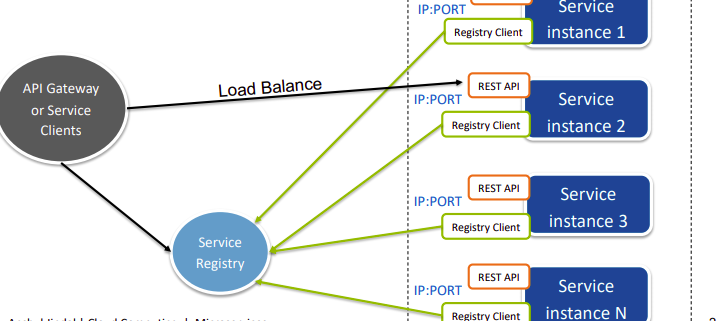
\includegraphics[width=0.7\textwidth]{client-side.png}
	\end{figure}
	
	
	\item \textbf{server-side} service discovery:
	\begin{itemize}
		\item an extra \textbf{load balancer}: it queries the registry and implements load balancing.
		
		$\rightarrow$ client has \textbf{no contact to service registry}
		
		$\rightarrow$ client \textbf{doesn't need to load balancing}
		
		\item Advantages:
		\begin{itemize}
			\item discovery abstracted away from client
			\item less code
		\end{itemize}
		Disadvantages: extra load balancer required
	\end{itemize}
	\begin{figure}[H]
		\centering
		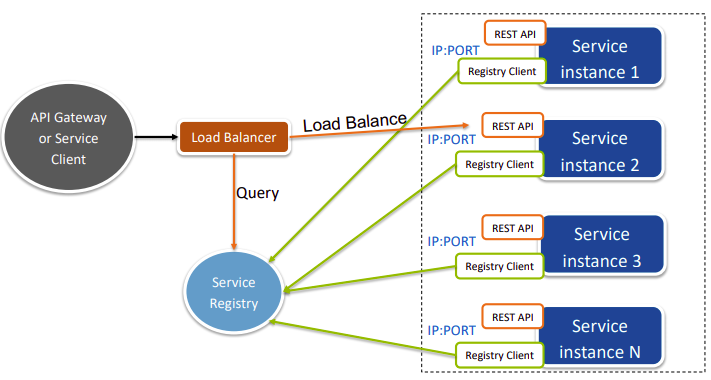
\includegraphics[width=0.7\textwidth]{server-side.png}
	\end{figure}
\end{itemize}

\subsubsection{Resilience -- Fault Tolerance Strategies}
\begin{itemize}
	\item basic request flow: 
	\begin{itemize}
		\item a user/load balancer sends a \textbf{request} to service and waits for a \textbf{response}.
		\item a \textbf{thread is assigned} along the request, in order to get data and send it back.
		\item when response is sent, the \textbf{thread is freed}. 
	\end{itemize}
	\begin{figure}[H]
		\centering
		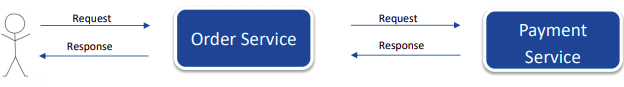
\includegraphics[width=0.8\textwidth]{request.png}
	\end{figure}
	\item \textbf{immediate failure}: fails at \textbf{request} (eg: connection refused) to service.
	\begin{itemize}
		\item possible reasons: overhead of requests
		\item solution: \textbf{try...catch}-code catches the error and returns error to client $\rightarrow$ thread is freed		
	\end{itemize}
	\begin{figure}[H]
		\centering
		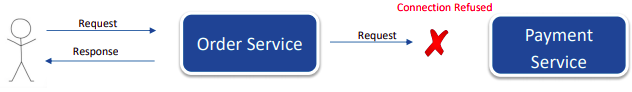
\includegraphics[width=0.8\textwidth]{immediate.png}
	\end{figure}
	
	
	\item \textbf{timeout failure}: fails at \textbf{response} from service to service. At high request rate, all threads are \textbf{waiting for response}, no free threads.
	\begin{itemize}
		\item possible reasons: service is overloaded or crashed
		
	\end{itemize}
	\begin{figure}[H]
		\centering
		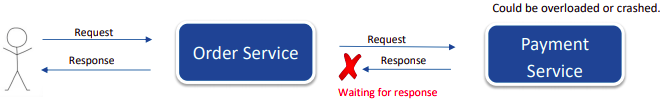
\includegraphics[width=0.8\textwidth]{timeout.png}
	\end{figure}
	
	\item \textbf{cascading failure}: due to timeout failure of one service instance to another service instance, this \textbf{timeout failure} is \textbf{propagated} to neighboured connected instances.
	\begin{figure}[H]
		\centering
		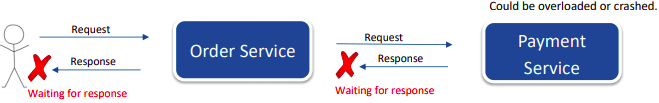
\includegraphics[width=0.8\textwidth]{cascading.png}
	\end{figure}
	\item Solutions to timeout/cascading failures: 
	\begin{itemize}
		\item timeout-value: returns error after timeout, thread is freed
		\item request interceptor/\textbf{circuit breaker}
		\begin{itemize}
			\item \textbf{intercepts all requests} from service to target service.
			\item \textbf{counter \& threshold implementation} of success \& failures. 
			\begin{itemize}
				\item closed: \#failures < threshold
				\item open: \#failures > threshold, default error response, thread is freed.
				\item half-open: remains open for a predefined sleep period and rechecks. 
			\end{itemize}
			\item checks regularly and refreshes.
		\end{itemize}
	\end{itemize}
	\begin{figure}[H]
		\centering
		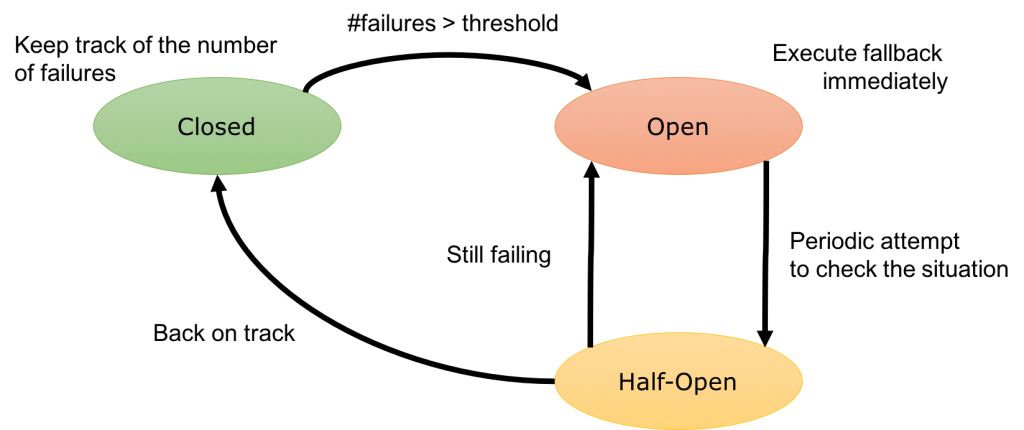
\includegraphics[width=0.7\textwidth]{circuit-breaker.png}
	\end{figure}
	
\end{itemize}

\subsubsection{Deployment Strategies}
\begin{itemize}
	\item \textbf{multiple service instances} per VM: service instances share resource of a VM together $\rightarrow$ for resource-efficient services
	\item \textbf{single service instance} per VM: for resource-hungry services
	\item \textbf{multiple service containers} per VM: each service instance is containerized with its needed libraries \& dependencies. $\rightarrow$ high portability, high scalability
	\item \textbf{single service container} per VM
\end{itemize}

\subsubsection{Rolling Updates Strategies}
\begin{itemize}
	\item Goal: implementation of updating of services.
	\item \textbf{Ramped-slow Rollout}: update in \textbf{rolling update} fashion. It \textbf{decreases old version} instances and \textbf{increases same number of new version} instances, until all old versions are removed.
	\begin{itemize}
		\item Advantages: 
		\begin{itemize}
			\item new version is slowly released across instances
			\item convenient for \textbf{stateful applications} that can handle rebalancing of data
		\end{itemize}
		Disadvantages:
		\begin{itemize}
			\item takes more time
			\item supporting mulitple APIs harder, if both versions use different patterns.
			\item no control over traffic, since load balancer directs request to either of the instances, it might follow wrong robin pattern.
		\end{itemize}
	\end{itemize}
	
	
	\item \textbf{Blue/Green}: new version of app is \textbf{deployed alongside} the old version. After testing new version, the load balancer will be \textbf{redirected} to send traffic to the new version. 
	
	\begin{itemize}
		\item Advantages:
		\begin{itemize}
			\item instant rollout/rollback
			\item no versioning issue (multiple versions coexist)
		\end{itemize}
		Disadvantages:
		\begin{itemize}
			\item requires double the resources. (same size of empty instances needed)
			\item requires testing before releasing, but still can't simulate the workload by client requests
		\end{itemize}
	\end{itemize}
	
	\item \textbf{Canary}: new version is \textbf{deployed and receives a subset of client requests} alongside the old version. We distribute the traffic amongst the versions by \textbf{adjusting the number of replicas} managed by a ReplicaSet.
	 After successful testing, all old versions are removed at one time.
	
	
	
	\begin{itemize}
		\item Advantages:
		\begin{itemize}
			\item version released for a subset of clients $\rightarrow$ testing of workload possible
			\item convenient for performance and error rate monitoring
			\item fast rollback 
		\end{itemize}
		Disadvantages:
		\begin{itemize}
			\item slow rollout: testing of workload, monitoring and improvement takes time
			\item fine tuned traffic distribution can be expensive. 
		\end{itemize}
	
	\end{itemize}
	
	\item \textbf{A/B Testing}: distribute traffic among versions \textbf{based on filter parameters} (weight, user, cookies). After successful testing, old versions are removed. 
	
	\begin{itemize}
		\item Advantages:
		\begin{itemize}
			\item intelligent load balancing
			\item full control over traffic distribution
		\end{itemize}
		Disadvantages:
		\begin{itemize}
			\item harder troubleshooting, distributed tracing of versions necessary
			\item additional tools needed
		\end{itemize}
		
		
		
	\end{itemize}
\end{itemize}
